
Results are shown from two sets of simulations in Figs. \ref{fig:15_candidate},\ref{fig:30_candidate}. Both of these figures show sum rate given in Eq. (\ref{eq:erg_sum_rate}) plotted vs. $\epsilon$. The left-hand side of the plots corresponds to more strict orthogonality (small $\epsilon$), while the right-hand side of the plot corresponds to more lax orthogonality (larger values of $\epsilon$)

The results shown in Fig. \ref{fig:15_candidate} are for $L = 15$. Results illustrated in this plot are broken into series that vary depending on $K$ and dimension of symbol constellation. The colour and shape of the datapoints in the series denotes the value of $K$: blue triangle for $K=2$, red square for $K=3$, and black circle for $K=4$. The fill of the datapoint denotes the dimension of constellation used for symbols: no fill corresponds to single dimensional (real) constellation (ie. BPSK, M-PAM), while solid fill corresponds to a two-dimensional (complex) constellation (ie. QPSK, M-QAM).

First we will discuss the data series belonging to two-dimensional constellations. From the plot we can see that there is a point of maxima for $0 < \epsilon < \infty$ in each of these curves. The location of this point of maxima agrees with expected results. The shape of these curves illustrates a tradeoff associated with choosing $\epsilon$: $\epsilon$ is best chosen such that it provides some degree of orthogonality between users to limit interference; however, it should not be so strict that we cannot find STAs to add to the SUS group that meet the orthogonality requirement. The portion of the curve to the left of the maximum is limited in terms of SUS group existence. The portion of the curve to the right of the maximum is limited in terms of interference. We can see that the curves with higher values of $K$ have a maximum associate with larger values of $\epsilon$ since we have a lower probability of finding a large number of STAs that meet strict orthogonality requirements. We can see that even though we are twice as many STAs with $K=4$ compared to $K=2$, the maximal sum rate is higher for $K=2$ than $K=4$. Although this result may seem counter-intuitive, consider the constraints being placed on these curves in terms of SUS group existence probability and interference. For $K=4,\ L = 15$ by the time existence probability is high enough to stop limiting sum rate, interference is high enough to limit the achievable sum rate below the $K=2$ case.

Next, consider the series corresponding to single-dimensional constellations. From these series we can see that lower values of $\epsilon$ are favorable. This is because the relaxed orthogonality requirement translates to a higher probability of SUS group existence, even for strict orthogonality requirements. We see  that the series for $K=4$ now has the largest maximum sum rate. Again, this is expected. Since the probability of SUS group existence has been significantly relaxed compared to the two-dimensional constellation case, the $K=4$ series is able to have a large enough existence probability at low interference to out-perform the $K=2$ series.

\begin{sidewaysfigure}
    \centering
    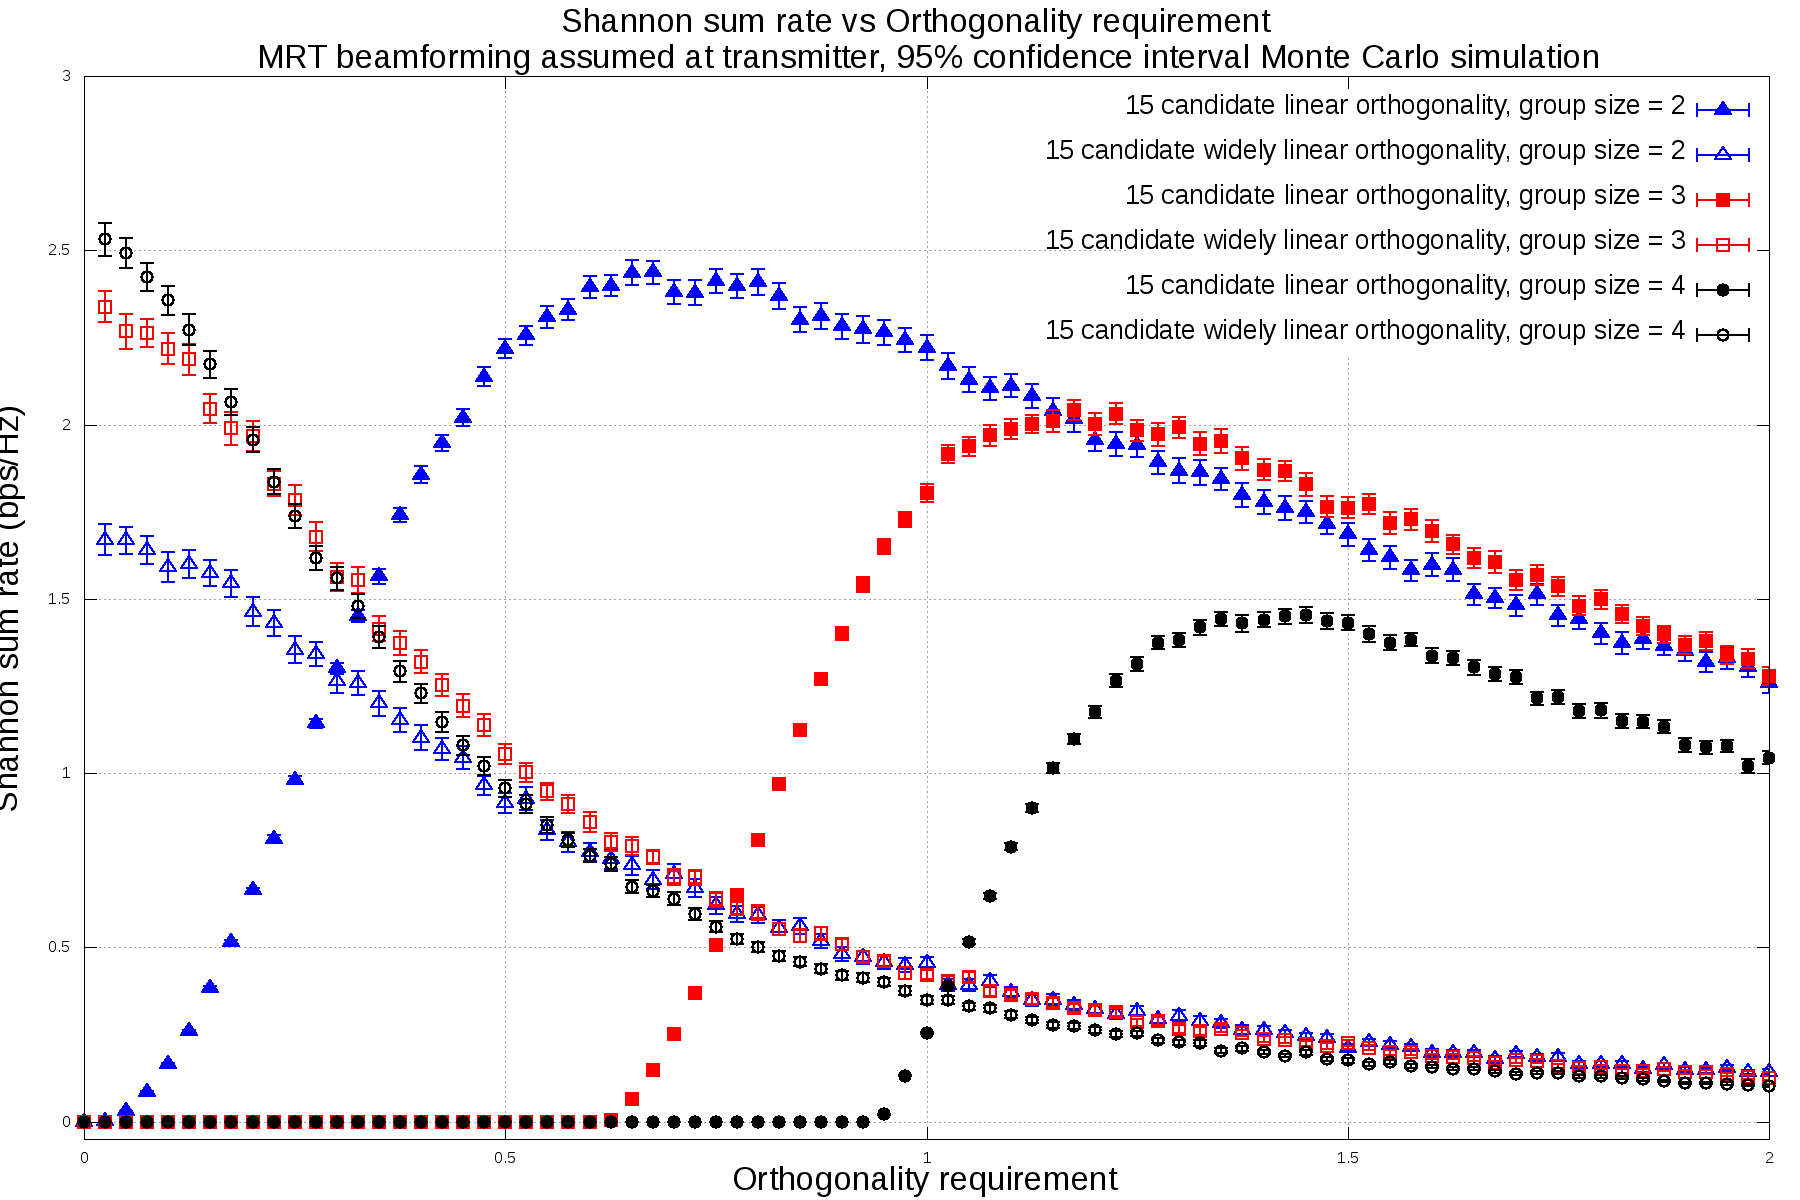
\includegraphics[width=24cm]{figs/15_candidate_mrt.png}\\
    \caption{Sum rate for single-dimensional and two-dimensional constellations, SUS group sizes set to 2, 3, 4. Number of candidate STAs for addition to SUS groups is held to 15.}
    \label{fig:15_candidate}
\end{sidewaysfigure}

Figure \ref{fig:30_candidate} shows  curves for two-dimensional constellation sum rates with $L = 30$ instead of 15. We see that the $K=3,4$ series now have higher maximum sum rate values. This result is expected: as the number of candidate STAs is increased, the probability of larger SUS groups existing for small values of $\epsilon$ increases. Increasing $L$ has less of an impact for $K=2$ because the existence probability has already saturated for small values of $\epsilon$.
\begin{sidewaysfigure}
    \centering
    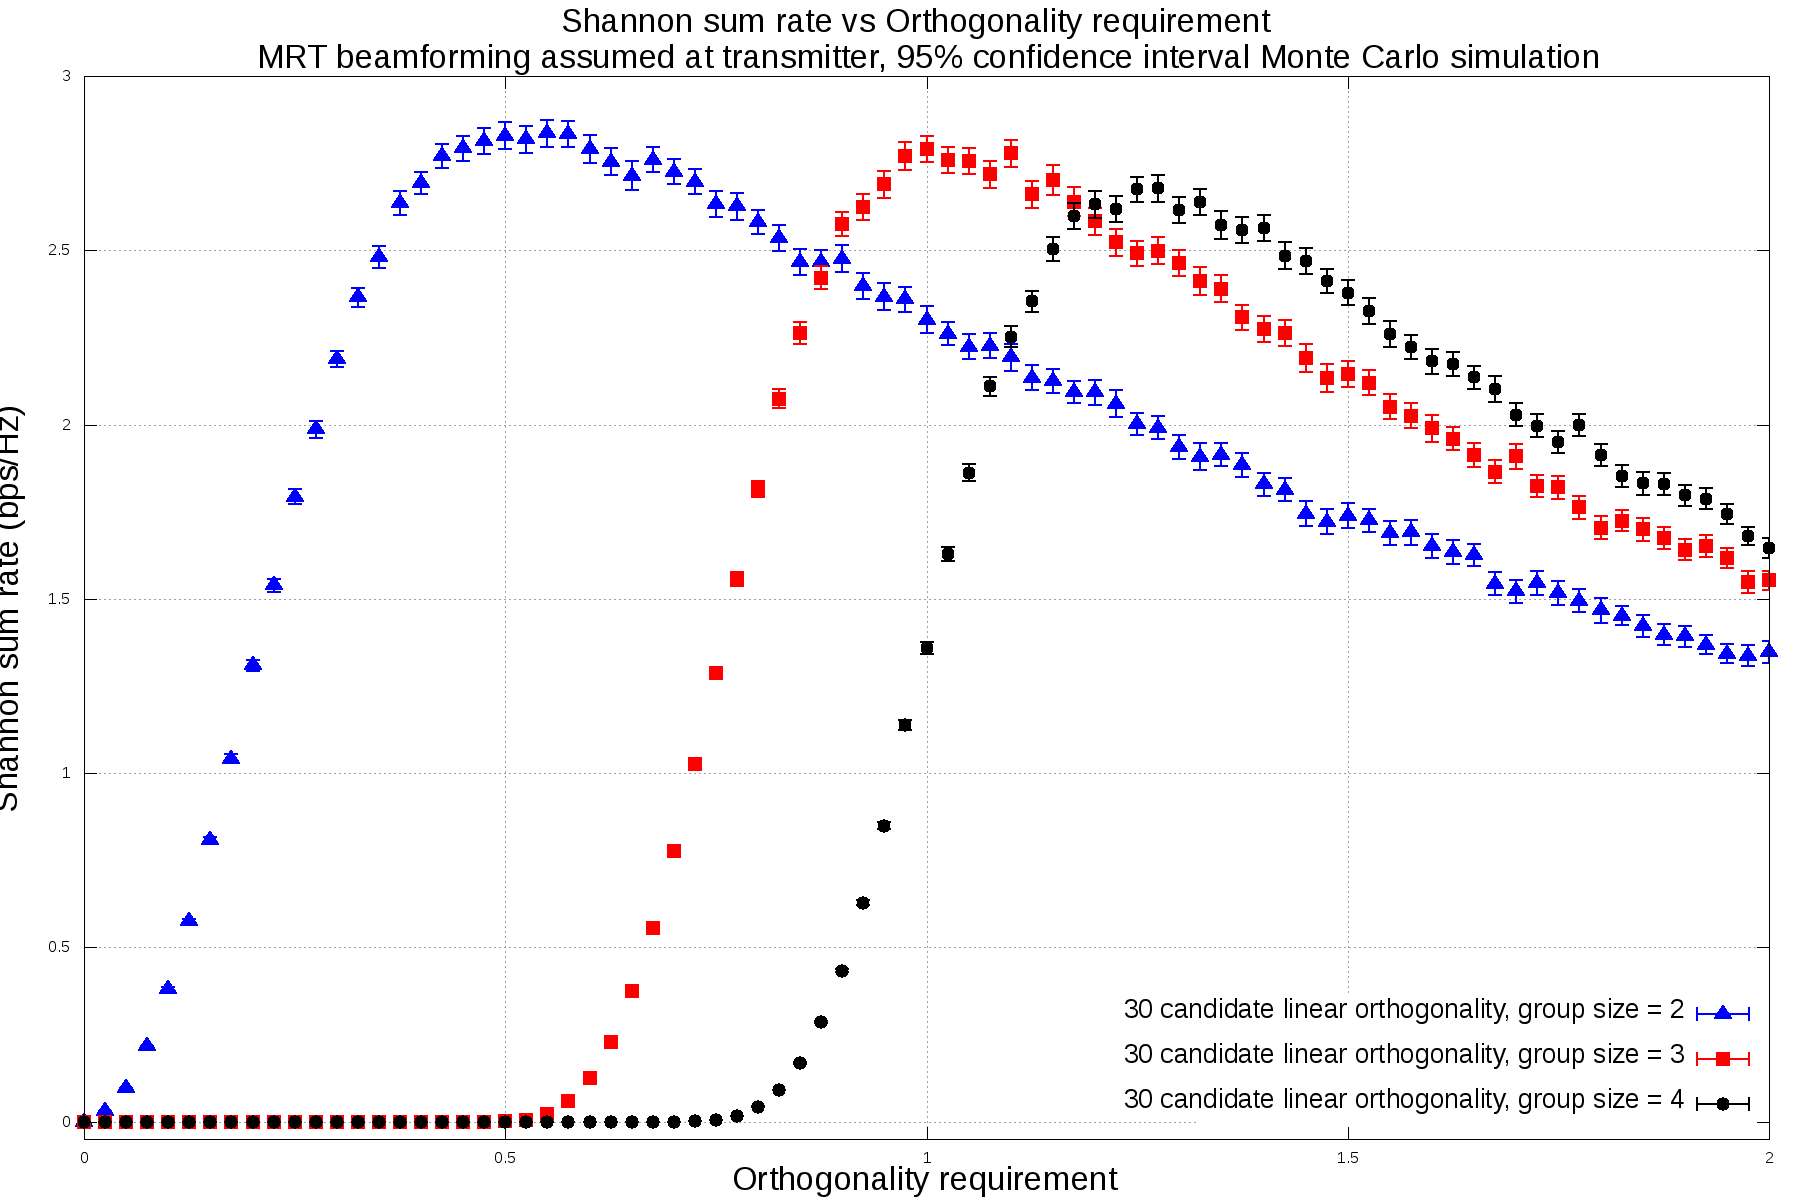
\includegraphics[width=24cm]{figs/30_candidate_mrt.png}\\
    \caption{Sum rate for two-dimensional constellations, SUS group sizes set to 2, 3, 4. Number of candidate STAs for addition to SUS groups is held to 30.}
    \label{fig:30_candidate}
\end{sidewaysfigure}
